%!TEX root=../sub_chapter_paper.tex

% \title{My famous Paper}
% \author{J. Doe$^{1}$, Co-author1$^{3,2}$}
% \affiliation{$^1$First affiliation\\$^2$Second affiliation\\$^3$Third affiliation}
% \pubStatus{DOI:XXXXX}
% \myabstract{
% \lipsum[8]
% }
% \keywords{Keyword 1, Keyword 2, ...}
% \mathsubclass{XXXXX, XXXXX} % comment this line if not appropriate

% \custommaketitle % use \custommaketitlenomath if \mathsubclass is not defined

\section{In-situ Thermal Annealing Platform}
\label{sec:In-situ Thermal Annealing Platform}

The deterministic generation of point defects in TMDs, such as sulfur vacancies, requires high thermal activation energy \cite{noh-2014,komsa-2015}. While conventional furnace annealing is widely used, it necessitates transferring samples through ambient conditions, which can lead to unintended oxidation or hydrocarbon re-contamination. Furthermore, the lack of in-situ optical monitoring during thermal treatment prevents precise control over defect density.

To overcome these challenges, we developed an in-situ local heating system integrated into a cryogenic photoluminescence (PL) setup. This system enables localized high-temperature annealing up to 1200~K under high vacuum ($<10^{-6}$~Torr), while maintaining the surrounding environment at cryogenic temperatures ($\sim$3.6~K).

Fig.~\ref{fig:annealing}(a) shows a photograph of the sample mounted inside the cryostat in front of a 50$\times$ objective. Fig.~\ref{fig:annealing}(b) illustrates the in-situ thermal annealing process. The system is based on a micro-heater chip that enables localized heating of the sample by applying an electrical current. The sample is placed directly on the chip, allowing controlled thermal annealing while maintaining the surrounding cryogenic environment.

During annealing, photoluminescence measurements can be performed simultaneously. Owing to the localized heating, the temperature of the cryostat remains low, enabling rapid cooling of the sample back to cryogenic temperature by simply switching off the current. This annealing and cooling sequence, together with optical measurements, is repeated at each target annealing temperature.

A key advantage of this configuration is that any adsorbates desorbed from the monolayer surface during annealing are immediately cryopumped onto the cold walls of the cryostat, rather than redepositing on the sample upon cooling. This effectively suppresses re-contamination between annealing steps and ensures that the optical response measured at cryogenic temperature reflects the intrinsic properties of the thermally treated material.

\begin{figure}[htbp]
	\centering
	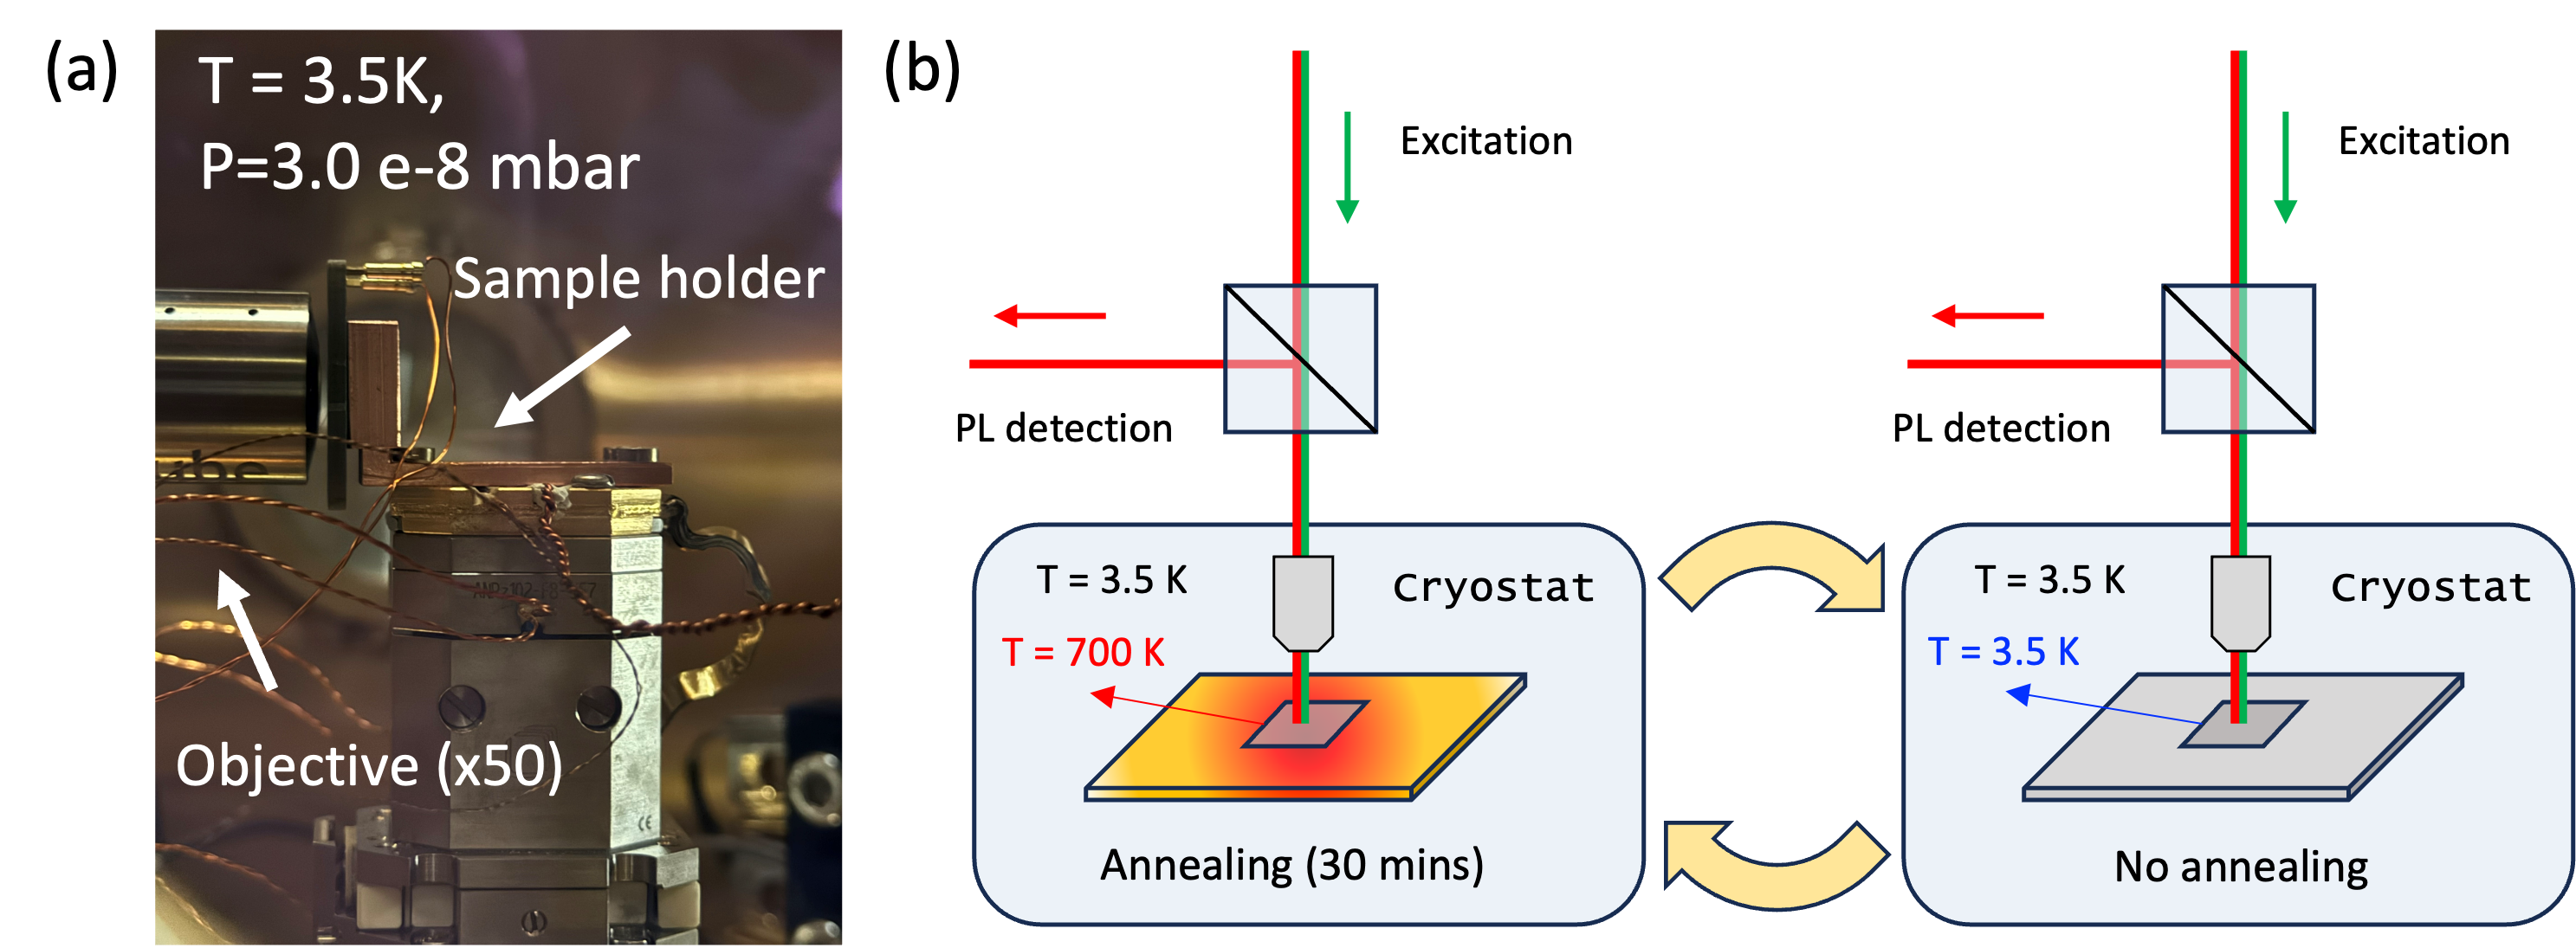
\includegraphics[width=\textwidth]{Figure/Chapter_three/annealing.png}
	\caption{(a) Photograph of the sample mounted inside the cryostat. (b) Schematic illustration of the in-situ thermal annealing process, where localized heating is applied to the sample while maintaining the surrounding cryogenic environment.}
	\label{fig:annealing}
\end{figure}



\section{Design and Characterization of the Micro-heater Chip}
\label{sec:Design and Characterization of the Micro-heater Chip}

The core of the in-situ thermal annealing platform is based on localized heating, which is enabled by a micro-heater chip. The micro-heater chips used in this work are commercial devices (EDEN Instruments) designed for localized heating applications, including transmission electron microscopy (TEM). The chip features a central region with an array of holes, allowing both thermal isolation and compatibility with optical and electron-beam measurements.

The chips are pre-calibrated by the manufacturer under secondary vacuum conditions at room temperature. As a result, calibration data relating temperature, electrical current, and resistance are provided together with the device.

Within the chip, a SiC membrane is suspended between two doped silicon contacts. Each contact is connected to external circuitry through gold electrodes on both sides. SiC was selected for its exceptional thermal stability and chemical inertness at elevated temperatures \cite{casady-1996,kimoto-2022}.

As illustrated in Fig.~\ref{fig:micro_heater}(a), the SiC membrane is resistive and undergoes localized heating when an electrical current is applied via Joule heating. An optical image of the chip is shown in Fig.~\ref{fig:micro_heater}(b).

The suspended membrane geometry provides high thermal resistance, effectively confining the heat to the central region where the sample is located. As the chip is calibrated at the center of the membrane, the temperature distribution is uniform in the central region around the array of holes, as shown in Fig.~\ref{fig:micro_heater}(c). In addition, blackbody radiation from the membrane is observed at temperatures around 1000$^\circ$C (Fig.~\ref{fig:micro_heater}(d)).

The heating process is controlled by applying a constant current while monitoring the corresponding voltage drop, allowing real-time tracking of the membrane resistance. The heating rate is carefully adjusted to avoid thermal stress in the hBN/TMD heterostructure.

\begin{figure}[htbp]
	\centering
	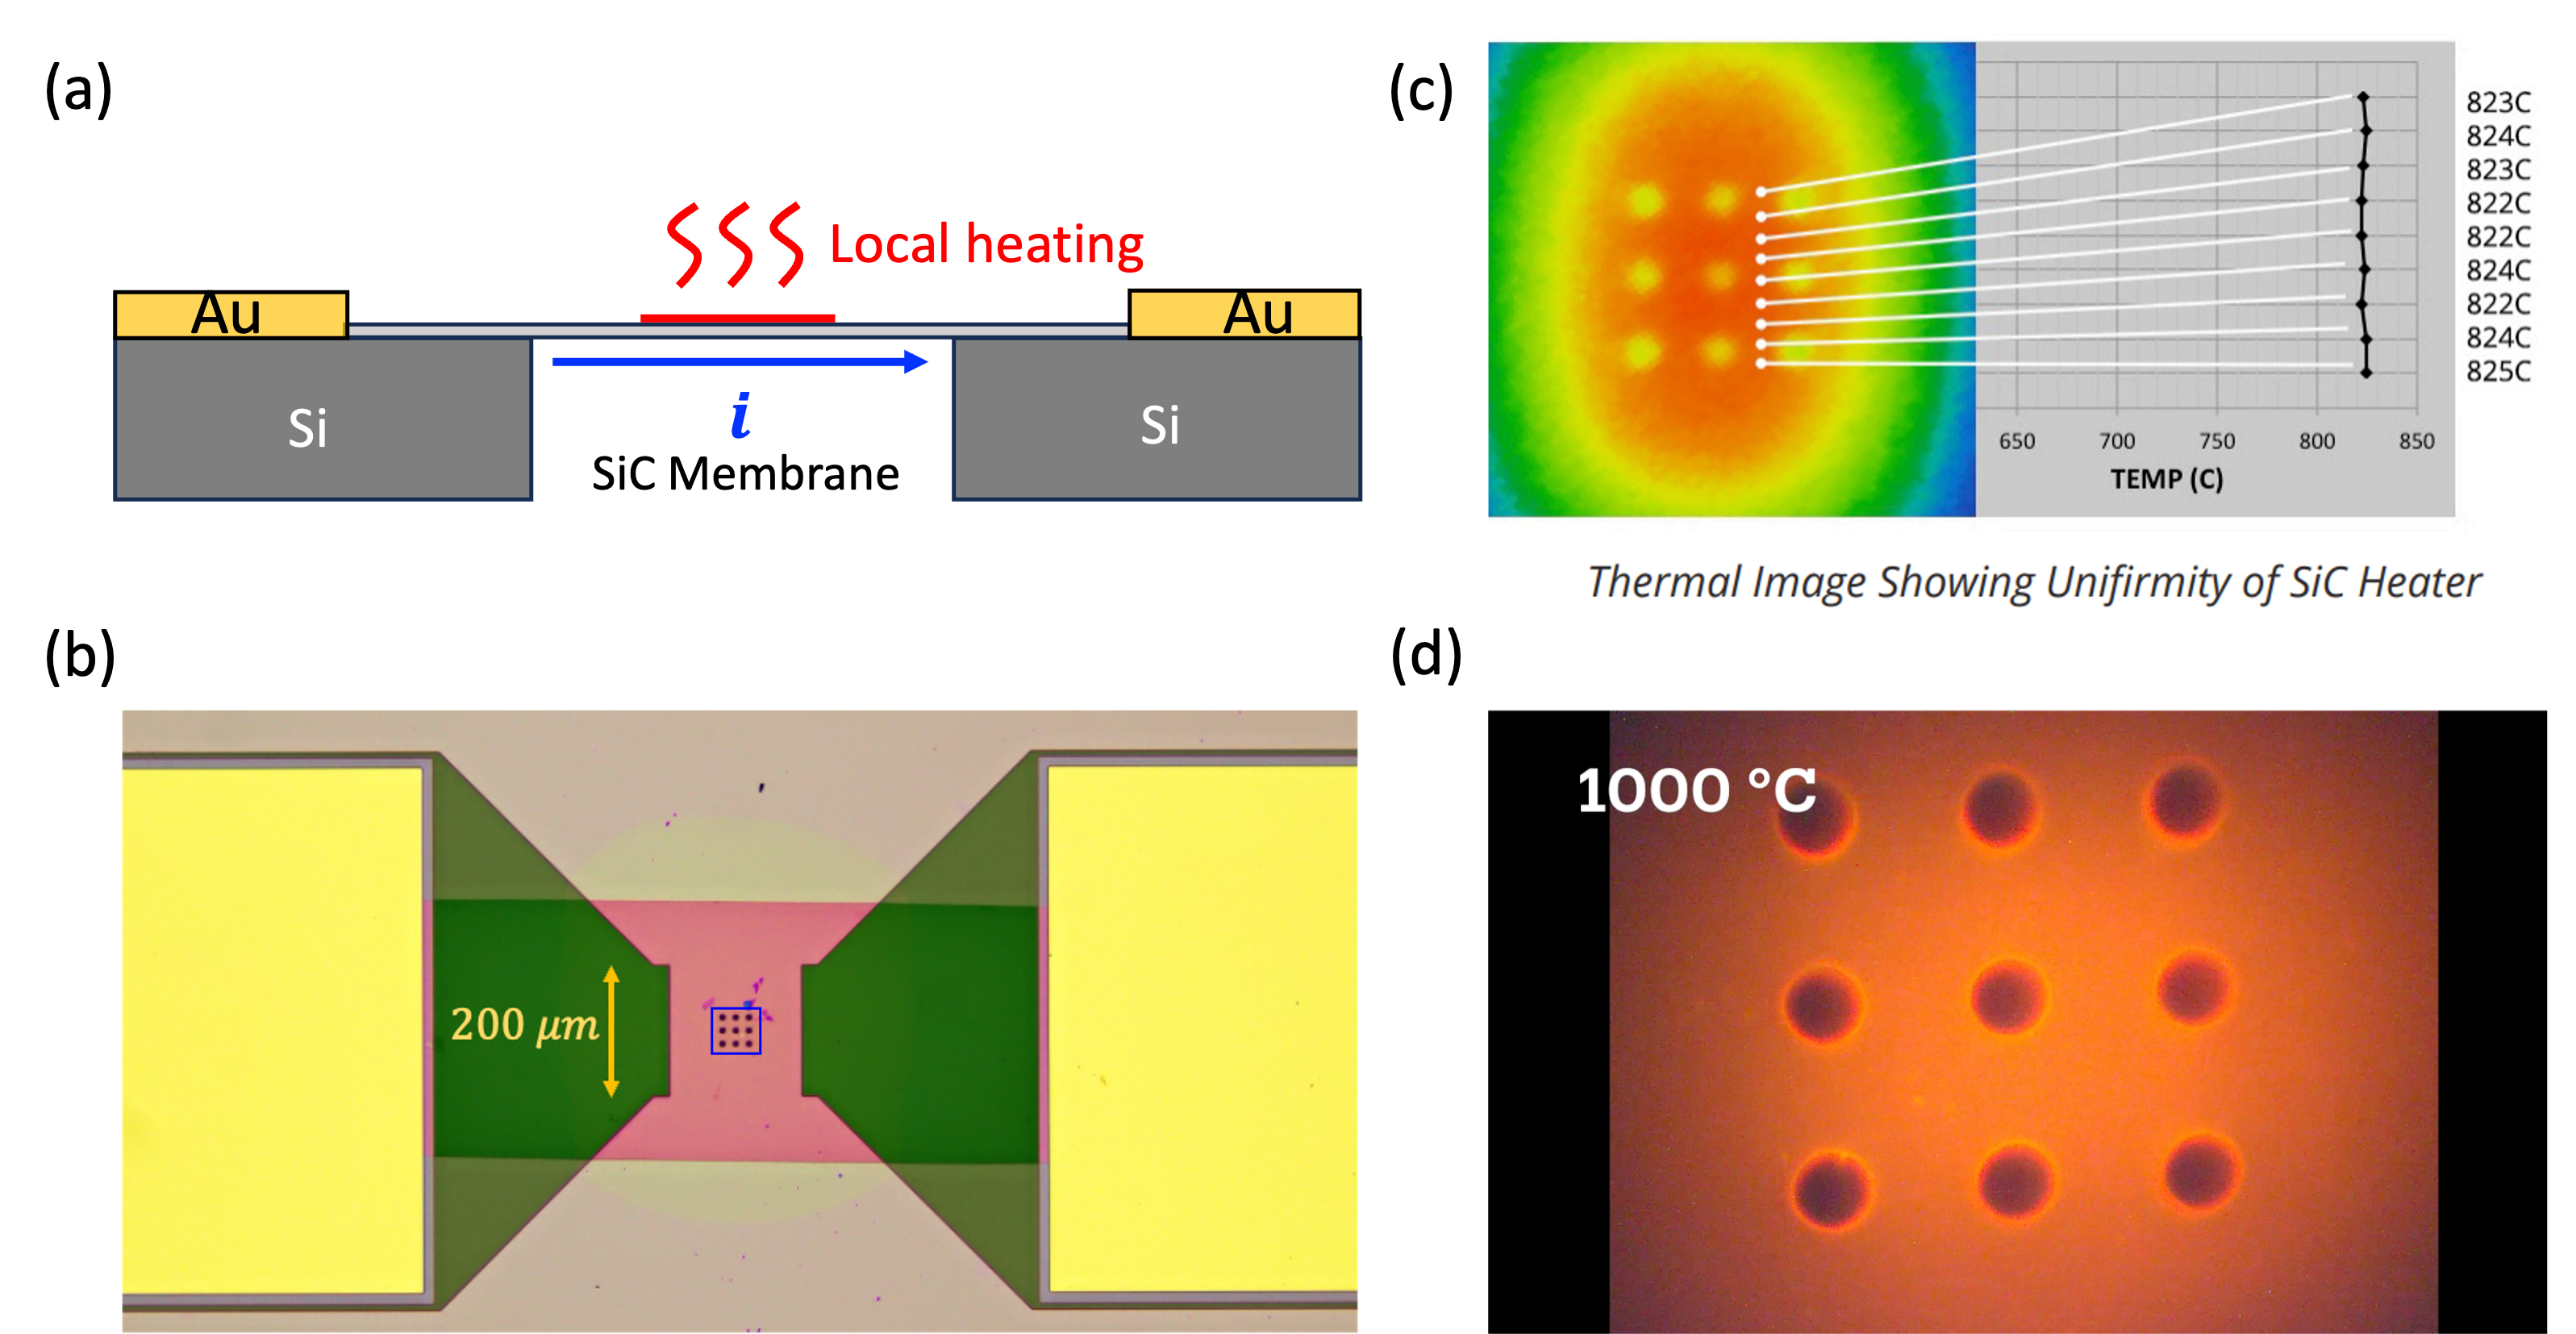
\includegraphics[width=\textwidth]{Figure/Chapter_three/micro_heater.png}
	\caption{(a) Schematic of the micro-heater chip illustrating localized heating driven by Joule heating. (b) Optical image of the chip (5$\times$ magnification). (c) Thermal image of the SiC heater showing uniform temperature distribution (provided by the manufacturer). (d) Optical image of blackbody radiation emitted from the SiC heater at temperatures around 1000$^\circ$C.}
	\label{fig:micro_heater}
\end{figure}

The SiC chip is mounted onto a custom-designed ceramic sample holder (Fig.~\ref{fig:heater_connection}(a)), which provides both mechanical support and electrical connectivity. Direct handling of the micro-heater chip with tweezers can easily damage the suspended membrane due to its mechanical fragility.

The mounting and bonding steps require careful handling. However, once the chip is securely attached to the holder and electrical connections are established, the assembly enables safe handling without direct contact with the fragile membrane. In practice, keeping the chip mounted on the holder facilitates reliable storage and repeated measurements.

In addition, the holder enables straightforward mounting and removal of the chip. The sample can be installed by inserting the copper support of the holder into the corresponding connector inside the cryostat, as shown in Fig.~\ref{fig:heater_connection}(b). Electrical connections between the chip terminals and the holder are established using aluminum wire bonding. This assembly is then interfaced with the internal wiring of the cryostat, which is connected to an external source-measure unit (SMU; Keithley 2400).

This configuration allows precise control of the electrical current supplied to the heater, while simultaneously monitoring the corresponding voltage and resistance. Overall, the ceramic holder provides reliable electrical interfacing while improving mechanical stability and handling.

Finally, after installation, the cryostat is sealed with a protective cover (Fig.~\ref{fig:heater_connection}(c)), enabling optical measurements under well-controlled thermal conditions at cryogenic temperatures.

\begin{figure}[htbp]
	\centering
	\includegraphics[width=\textwidth]{Figure/Chapter_three/heater_connection.png}
	\caption{(a) Micro-heater chip mounted on a custom-designed ceramic sample holder. (b) Sample holder installed inside the cryostat in front of the objective. (c) Cryostat with the protective cover closed, enclosing the objective and electrical connections.}
	\label{fig:heater_connection}
\end{figure}



% section introduction (end)

\section{Temperature Calibration}
\label{sec:Temperature Calibration}

Precise temperature control is essential for correlating annealing conditions with defect formation. In particular, it is necessary to determine the temperature at which defect-related phenomena emerge.

As discussed in Sec.~\ref{sec:Design and Characterization of the Micro-heater Chip}, the micro-heater chip is pre-calibrated by the manufacturer under vacuum conditions at room temperature. Under these conditions, the temperature can be accurately controlled based on the provided calibration data, which relates electrical current, voltage, and resistance to temperature.

However, in the present system, the micro-heater chip is integrated into a cryogenic environment. During operation, the chip is locally heated while the surrounding cryostat remains at low temperature. In this configuration, the manufacturer-provided calibration is no longer directly applicable, and the actual temperature of the sample cannot be reliably determined from electrical parameters alone.

Therefore, an independent calibration method is required to establish a reliable temperature scale under experimental conditions. We introduce two complementary spectroscopic thermometers that together cover the full annealing range used in this work: the neutral exciton emission energy of WS$_2$ (valid from 3.6~K to $\sim$925~K) and the blackbody radiation spectrum of the SiC membrane (valid above $\sim$900~K).

\subsection{Temperature Calibration Based on Exciton Emission Energy}
\label{subsec:calibration_exciton}

We employ an optical method based on photoluminescence (PL) spectroscopy. Monolayer TMDs such as WS$_2$ exhibit strong light emission due to their direct bandgap electronic structure, enabling precise tracking of their emission energy.

The emission energy of the neutral exciton ($X_A^0$) is strongly dependent on temperature. This dependence originates from temperature-induced bandgap renormalization in semiconductors, primarily driven by electron--phonon interactions. As the temperature increases, the bandgap decreases, resulting in a redshift of the PL emission. This well-defined energy shift allows the exciton emission to serve as a reliable indicator of the local temperature.

This temperature dependence of the exciton energy can be described using an analytical model known as the P\"{a}ssler model \cite{passler-1997}:

\begin{equation}
E_g(T) = E_g(0) - \frac{\alpha \Theta}{2}
\left[
\sqrt[p]{1 + \left(\frac{2T}{\Theta}\right)^p} - 1
\right]
\end{equation}

where the parameters for an encapsulated sample were determined in \cite{nagler-2018} and are given by $E_g(0) \approx 2.063\,\mathrm{eV}$, $\alpha \approx 3.47 \times 10^{-4}\,\mathrm{eV/K}$, $\Theta \approx 200.89\,\mathrm{K}$, and $p \approx 2.35$.

Fig.~\ref{fig:calibration_rt} shows the evolution of the PL spectrum of a WS$_2$ monolayer with increasing temperature under vacuum conditions. At room temperature, the PL spectrum consists of one or two dominant peaks corresponding to the neutral exciton and the negatively charged exciton, enabling straightforward tracking of the exciton emission energy.

As the temperature increases, a clear redshift of the exciton energy is observed (Fig.~\ref{fig:calibration_rt}(a)). The measured energy shift is in excellent agreement with the P\"{a}ssler model, as shown in Fig.~\ref{fig:calibration_rt}(b). In addition, a shift of approximately 19~meV is attributed to the difference in exciton binding energy between encapsulated and non-encapsulated monolayers \cite{raja-2017,cadiz-2017}.

From these calibration results, a direct relationship between temperature and exciton emission energy is established. Consequently, the exciton energy can be used to estimate the local temperature of the emitter, in this case a monolayer TMD.

\begin{figure}[htbp]
	\centering
	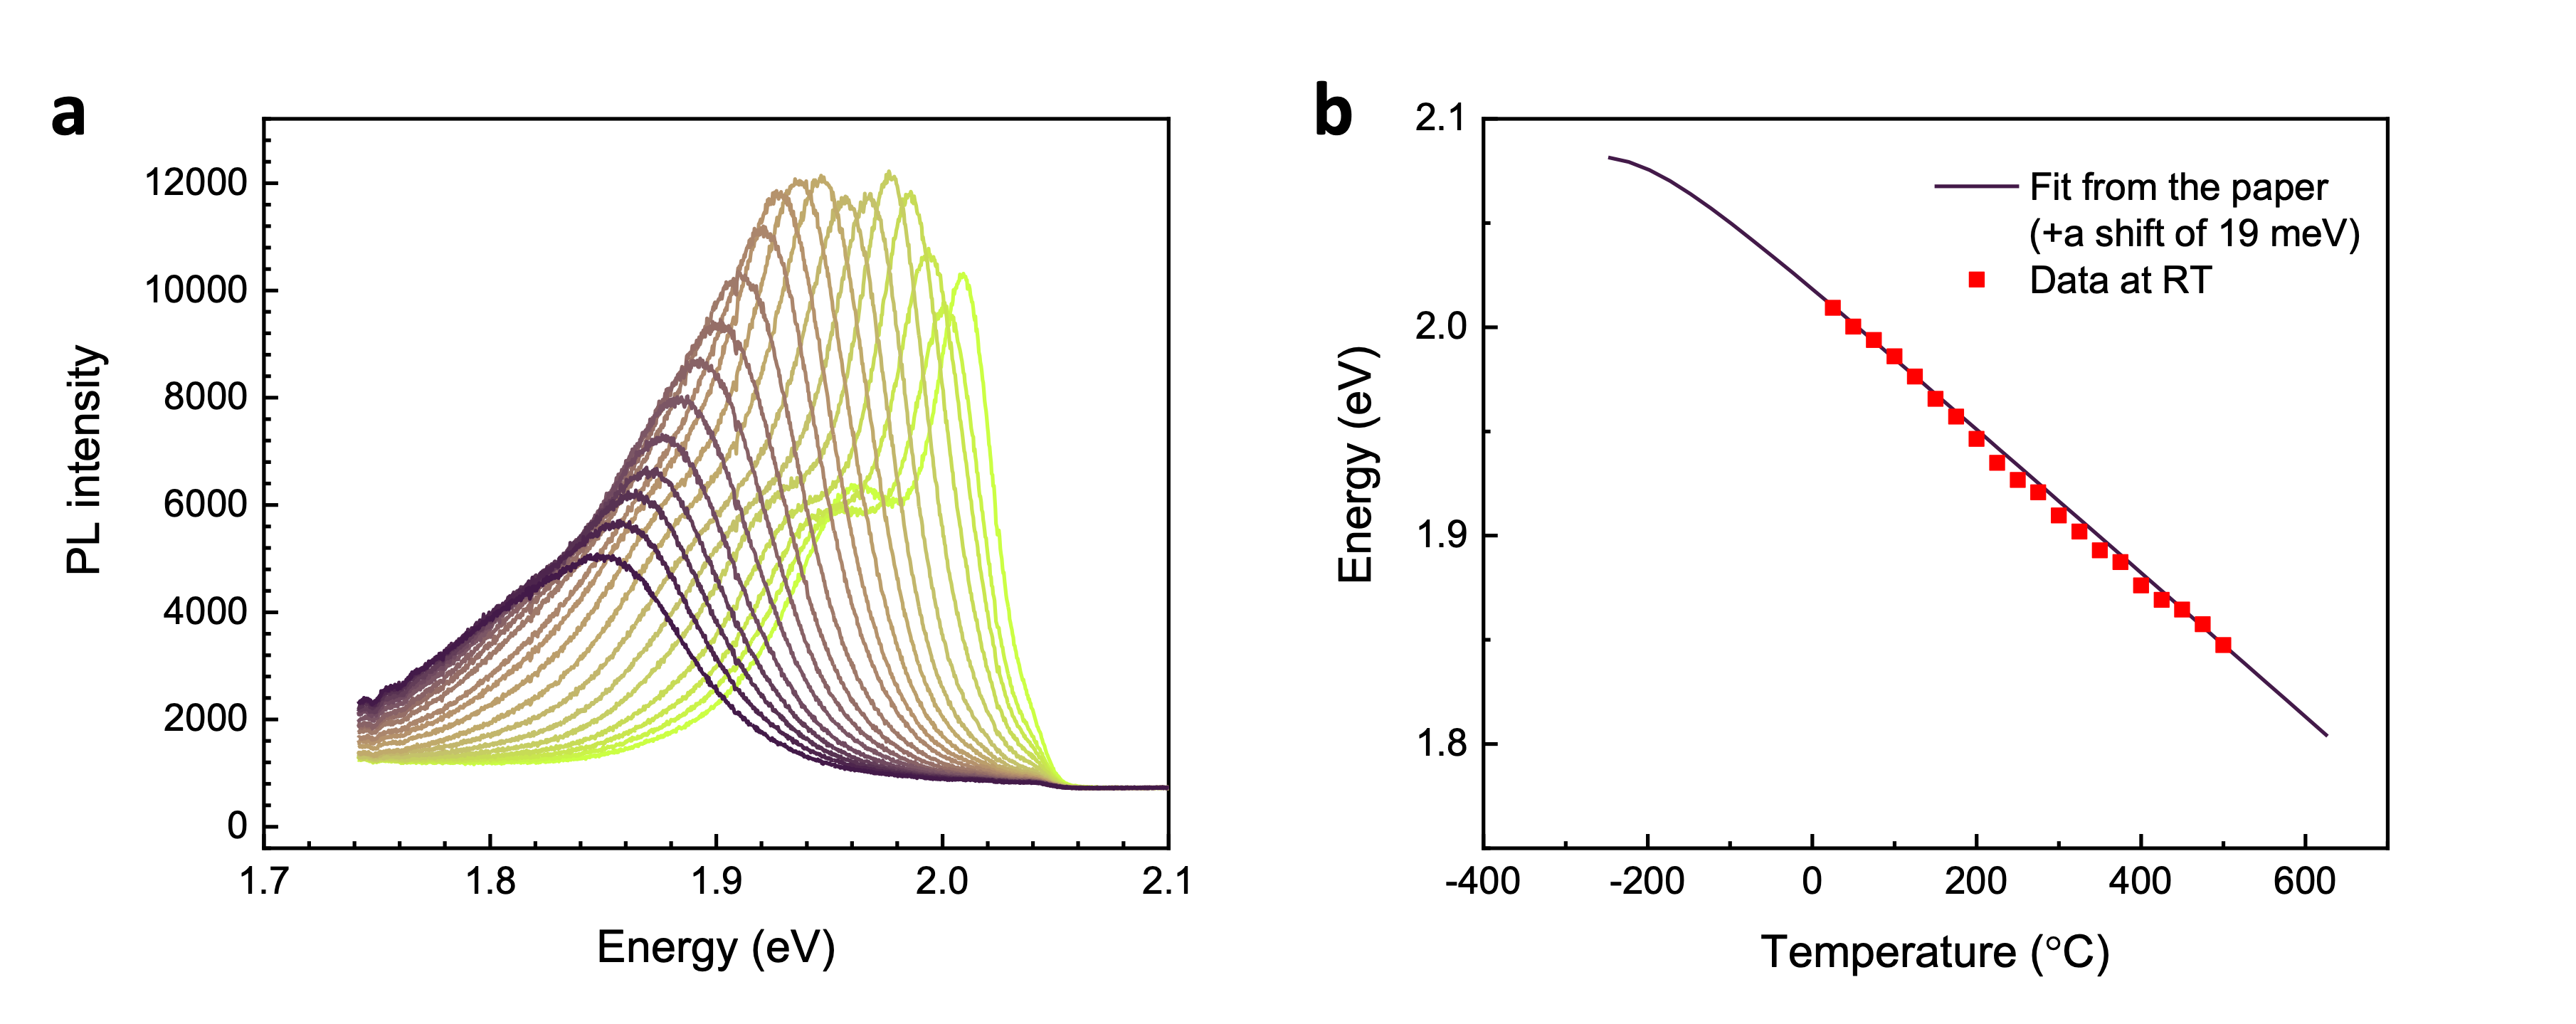
\includegraphics[width=\textwidth]{Figure/Chapter_three/calibration_rt.png}
	\caption{(a) Evolution of the PL spectrum of a WS$_2$ monolayer from 25$^\circ$C (300 K) to 500$^\circ$C (773 K). (b) Temperature dependence of the neutral exciton ($X_A^0$) energy and its fit using the P\"{a}ssler model.}
	\label{fig:calibration_rt}
\end{figure}

To further validate this approach over a wide temperature range, additional measurements were performed in a cryostat at temperatures below room temperature. In encapsulated WS$_2$ monolayers, the neutral exciton emission is significantly suppressed at low temperatures due to the presence of a lower-energy dark excitonic state arising from spin--valley coupling in the band structure. Furthermore, in non-encapsulated WS$_2$ monolayers, dielectric disorder in the surrounding environment leads to a PL spectrum containing multiple excitonic complexes that cannot be clearly identified. As a result, direct PL measurements become less reliable in this regime.

To overcome this limitation, photoluminescence excitation (PLE) spectroscopy was employed. By tuning the excitation energy and probing the absorption resonance, both A and B exciton resonances could be reliably tracked over the temperature range from 3~K to 300~K using the cryostat temperature control system. The evolution of the PLE spectra is shown in Fig.~\ref{fig:calibration_PLE}. The extracted exciton energies from PLE measurements are also in good agreement with the P\"{a}ssler model.

When comparing PL and PLE at 300~K, only a small energy difference of a few meV is observed, which can be attributed to the Stokes shift.

\begin{figure}[htbp]
	\centering
	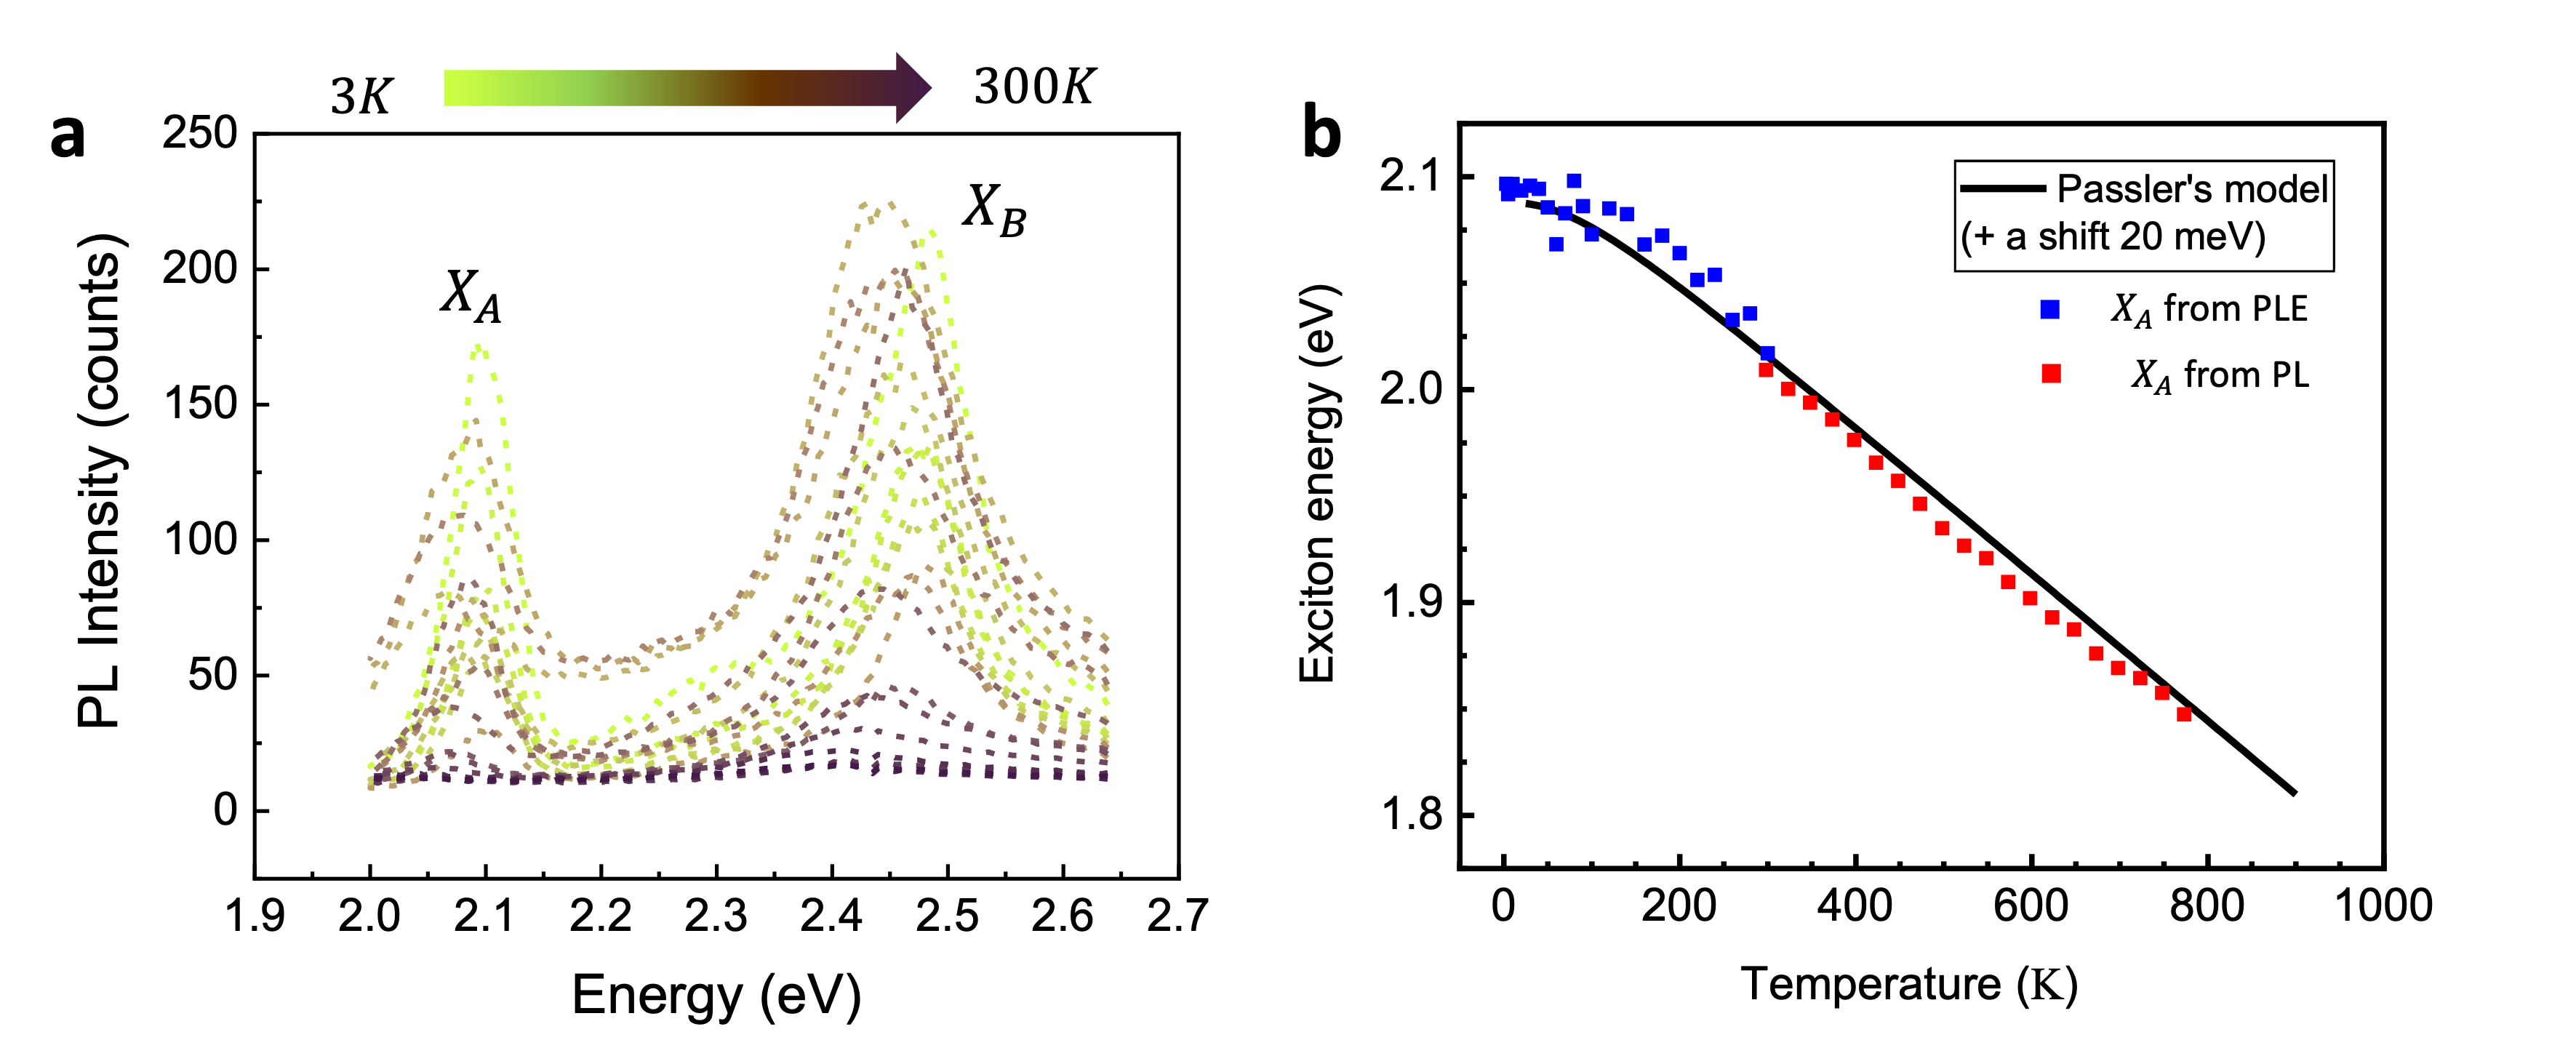
\includegraphics[width=\textwidth]{Figure/Chapter_three/calibration_PLE.png}
	\caption{(a) Evolution of the PLE spectrum of a WS$_2$ monolayer from 3~K to 300~K. (b) Temperature dependence of the neutral exciton ($X_A^0$) energy obtained from PL and PLE measurements, along with the P\"{a}ssler model fit.}
	\label{fig:calibration_PLE}
\end{figure}

By combining cryostat-based temperature control at low temperatures and micro-heater-induced local heating at higher temperatures, the exciton energy was tracked over a broad temperature range, confirming its robustness as a temperature indicator.

\subsection{Local Temperature Estimation Using Exciton Energy}
\label{subsec:calibration_local}

Having established exciton emission energy as a temperature indicator, we now use it to estimate the local temperature during in-situ annealing in a cryogenic condition.

In practice, the electrical current applied to the micro-heater is gradually increased while simultaneously recording the PL spectrum. The evolution of the neutral exciton ($X_A^0$) energy is monitored in real time. Using the previously established relationship between exciton energy and temperature, the measured exciton energy is converted into the corresponding local temperature of the sample.

We first applied this approach to non-encapsulated WS$_2$ monolayers over a broad annealing range. However, at elevated temperatures, the PL intensity decreases significantly, making it difficult to reliably extract the exciton energy.

More robust measurements were obtained using hBN-encapsulated WS$_2$ monolayers. In this case, the PL spectra remain well-defined up to temperatures of approximately 925~K, as shown in Fig.~\ref{fig:pl_evolution}(a,b). A continuous redshift of the exciton energy is observed as the heating current is increased, demonstrating that the exciton energy can be used to track the local temperature during in-situ annealing. The PL intensity decreases monotonically with temperature [Fig.~\ref{fig:pl_evolution}(c)], reflecting the activation of non-radiative recombination channels at elevated temperatures.

\begin{figure}[htbp]
	\centering
	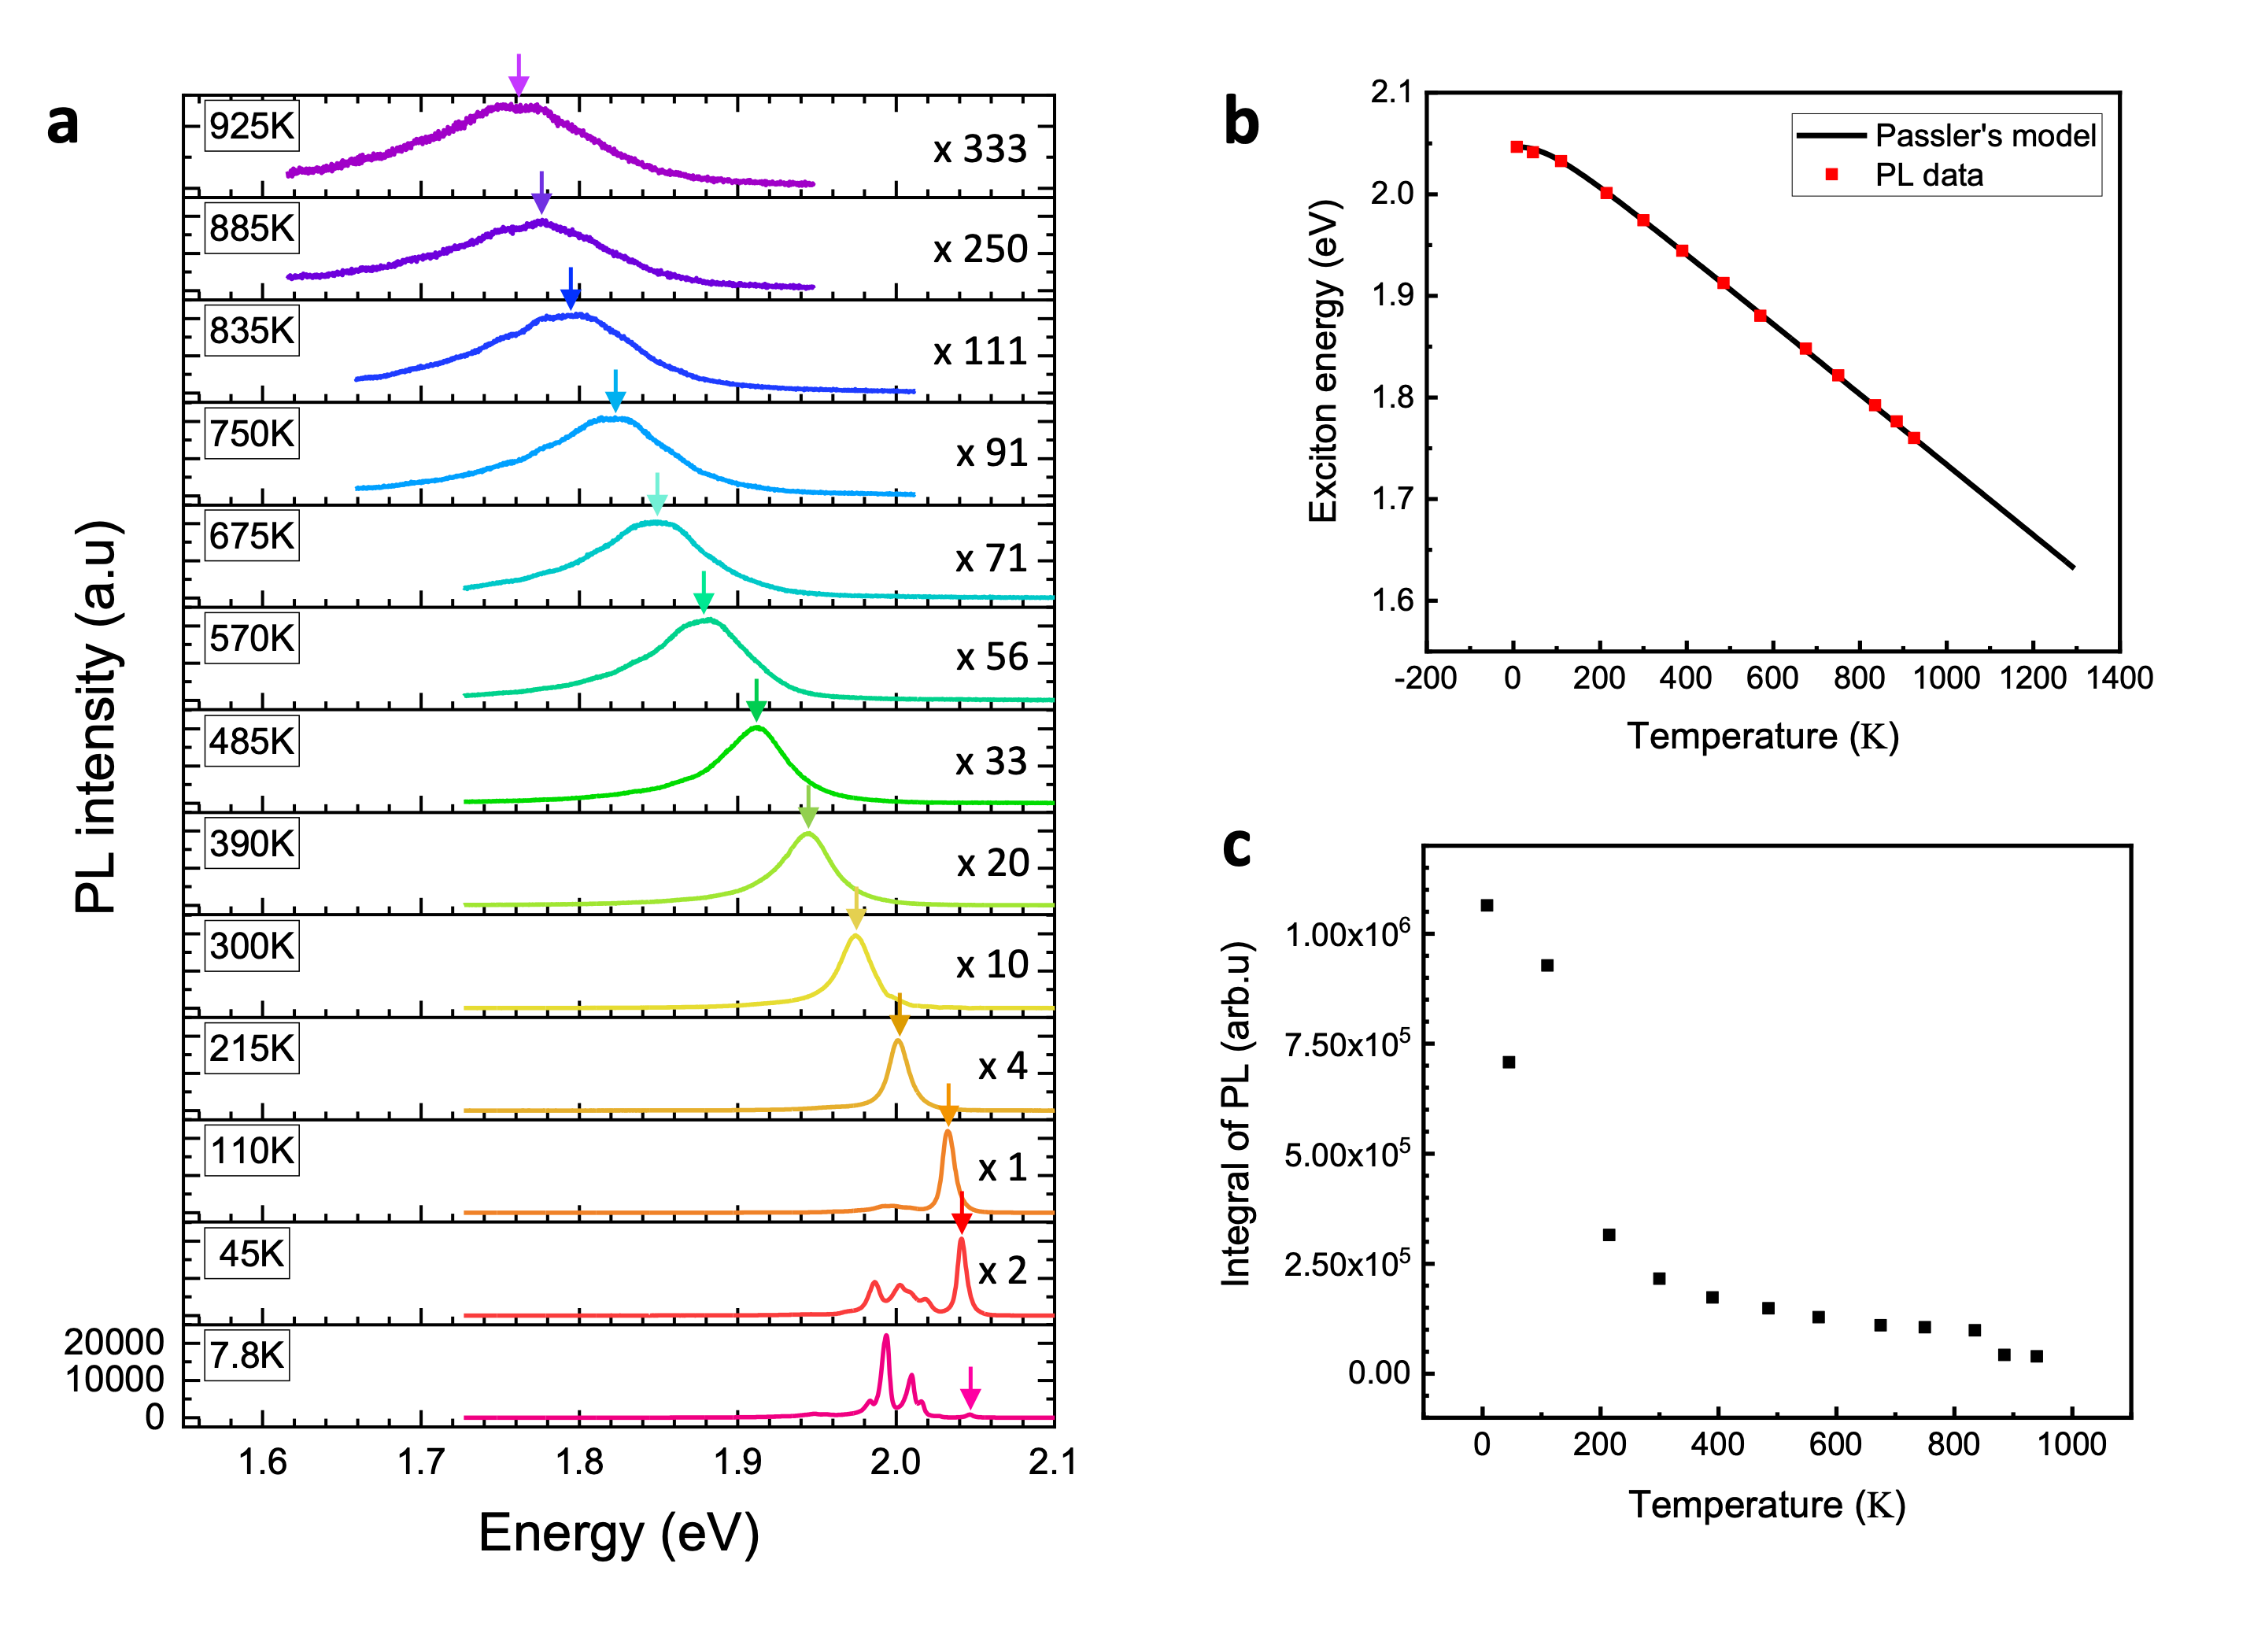
\includegraphics[width=\textwidth]{Figure/Chapter_three/pl_evolution.png}
	\caption{(a) Evolution of the PL spectrum of a WS$_2$ monolayer from 7.8~K to 925~K. (b) Temperature dependence of the neutral exciton ($X_A^0$) energy obtained from PL, along with the P\"{a}ssler model fit. (c) Temperature dependence of integrated PL intensity.}
	\label{fig:pl_evolution}
\end{figure}

\subsection{Extended Calibration Using Blackbody Radiation}
\label{subsec:calibration_blackbody}

At temperatures above $\sim$925~K, the PL intensity becomes too weak to extract a reliable exciton peak position. In this high-temperature regime, the SiC membrane itself emits detectable blackbody radiation in the visible range. By turning off the excitation laser and recording the thermal emission spectrum of the membrane, the temperature can be extracted by fitting to Planck's law:

\begin{equation}
B(\nu, T) = A \frac{(h\nu)^2}{e^{h\nu / k_B T} - 1}
\end{equation}

where $A$ is a proportionality constant that accounts for the spectral response of the detection system, corrected by an independently measured efficiency curve. At 925~K (determined from the exciton position), the blackbody fit yields $924 \pm 3.4$~K—a discrepancy of less than 1~K—confirming excellent agreement between the two thermometers at the crossover temperature.

At higher temperatures where the excitonic PL is no longer detectable, blackbody radiation serves as the sole thermometer. The temperature--power relationship extracted from this calibration is approximately linear, enabling interpolation between measured calibration points. Together, the two methods provide reliable temperature determination across the full annealing range from 3.6~K to $\sim$1500~K.

All temperatures quoted in Chapter~\ref{chap:chapter_four} refer to the temperature of the SiC membrane during the annealing step, as determined by this combined calibration protocol.



\section{Stability and Reproducibility of Local Annealing}
\label{sec:Stability and Reproducibility of Local Annealing}

A critical requirement for systematic defect engineering is that the annealing platform deliver reproducible results: the same annealing temperature applied to different samples should produce consistent changes in the PL spectrum, and the spatial position of the laser spot relative to the sample should remain stable across multiple thermal cycles.

\subsection{Spatial Stability Under Thermal Cycling}
\label{subsec:stability_spatial}

Optical images of the SiC membrane were recorded at 1000$^\circ$C and again after cooling back to room temperature. Comparison of the two images reveals a lateral displacement of less than 1~$\mu$m, which is below the diffraction-limited laser spot size used in our measurements ($\sim$1~$\mu$m). This remarkable positional stability arises from the symmetric mechanical design of the suspended membrane and the absence of large thermal gradients across the silicon support frame.

As a result, the laser spot can be reliably repositioned to the same location on the monolayer after each annealing step, enabling the PL spectrum of a single fixed spot to be tracked throughout the entire annealing sequence. This is essential for unambiguously attributing spectral changes to the thermal treatment rather than to spatial inhomogeneities in the sample.

\subsection{Thermal Dissociation Limit of WS\textsubscript{2}}
\label{subsec:stability_dissociation}

To establish the upper bound of safe annealing temperature, Raman spectroscopy was performed on a WS$_2$ monolayer during continuous heating from 25$^\circ$C to 1000$^\circ$C under vacuum. Both the E$_{2g}$ (in-plane) and A$_{1g}$ (out-of-plane) Raman modes were monitored. Both peaks redshift with increasing temperature, with the A$_{1g}$ mode shifting at a rate of $-0.0134$~cm$^{-1}$/K, and both eventually vanish at approximately 1000$^\circ$C (1273~K). Optical microscopy after annealing to 1200$^\circ$C confirms that the monolayer is no longer visible under white-light illumination, consistent with the thermal dissociation temperature of WS$_2$ in vacuum reported by Brainard \cite{brainard-1968} at approximately 1313~K.

On the basis of these results, all annealing experiments in this thesis were performed at temperatures below 1273~K. A standard annealing step consists of increasing the current gradually to the target value, holding for 30~minutes, and then reducing the current slowly until the membrane returns to the cryostat base temperature. The 30-minute hold time was found to be sufficient for the PL spectrum to reach a stable state at each temperature, as verified by monitoring the PL in real time during the hold period.

\subsection{Reproducibility Across Chips}
\label{subsec:stability_reproducibility}

The annealing protocol was applied to more than five independently fabricated encapsulated samples mounted on different micro-heater chips. In all cases, the PL spectra before annealing showed comparable optical quality, with excitonic linewidths of a few meV consistent with high-quality hBN encapsulation. The temperature at which defect-related emission first appears varies by $\pm$50--100~K between samples, reflecting differences in the initial defect density of the as-exfoliated monolayers and local variations in the strain state of the heterostructure on the membrane. Despite this sample-to-sample variability in threshold temperature, the spectral characteristics of the defect emission—linewidth, extra binding energy, and power-dependent saturation—are reproducible across all samples in which it was observed. This reproducibility confirms that the in-situ annealing platform generates defects through a reliable thermally activated mechanism rather than stochastic damage.

% ---- bibliography

\printbibliography[heading=subbibintoc]
% \bibliographystyle{apalike}
% \bibliography{bib_thesis}
